После запуска приложения в главном окне будет предложено осуществить вход от имени пользователя (рис.~\ref{main_win_patient:main_win_patient}) или администратора (рис.~\ref{main_window_admin:main_window_admin}).

\begin{figure}[h!]
\center{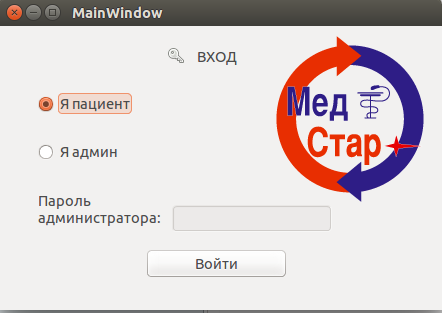
\includegraphics[width=0.5\linewidth]{main_win_patient}}
\caption{Вход от имени пользователя}
\label{main_win_patient:main_win_patient}
\end{figure}

\begin{figure}[h!]
\center{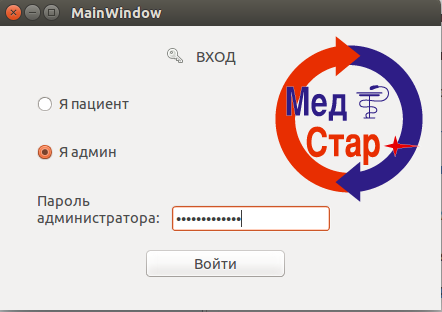
\includegraphics[width=0.5\linewidth]{main_window_admin}}
\caption{Вход от имени администратора}
\label{main_window_admin:main_window_admin}
\end{figure}
 
После нажатия кнопки <<Войти>> от лица пациента появится окно для записи на прием (рис.~\ref{enroll:enroll}). 
Если пациент еще не зарегистрирован в базе данных, то ему будет предложено пройти регистрацию (рис.~\ref{register_win:register_win}). После чего необходимо повторно нажать кнопку <<Записаться>> в окне для записи на прием. В результате будет успешно добавлен и сгенерирован в формате PDF талон на прием к специалисту (рис.~\ref{talon:talon}).

\begin{figure}[h!]
\center{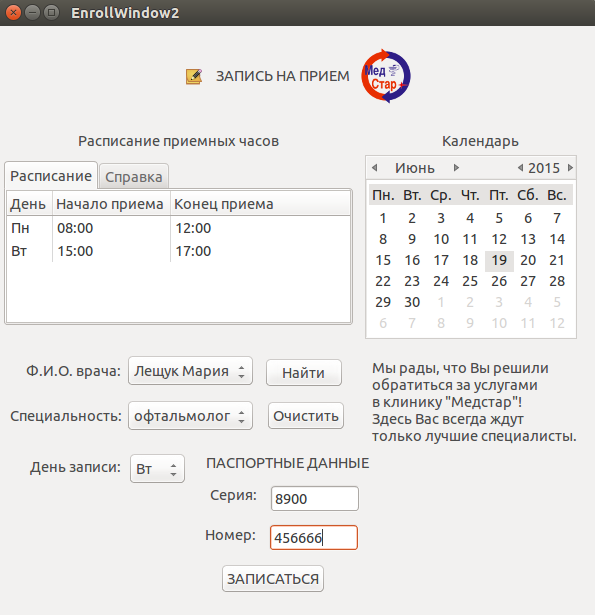
\includegraphics[width=0.9\linewidth]{enroll}}
\caption{Окно для записи на прием}
\label{enroll:enroll}
\end{figure}

\begin{figure}[h!]
\center{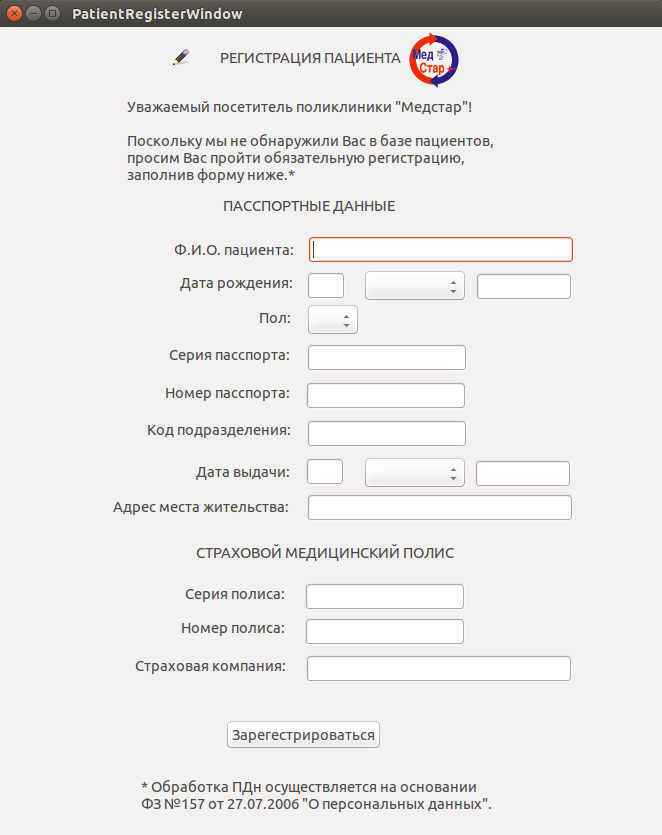
\includegraphics[width=0.9\linewidth]{register_win}}
\caption{Окно регистрации}
\label{register_win:register_win}
\end{figure}

\begin{figure}[h!]
\center{
\includegraphics[width=0.9\linewidth]{talon}}
\caption{Талон пациента}
\label{talon:talon}
\end{figure}

После нажатия кнопки <<Войти>> от лица администратора и успешного ввода пароля станет доступно окно управления базой данных. Оно позволяет как просматривать данные в таблицах (рис.~\ref{admin_find:admin_find}), так и добавлять (рис.~\ref{admin_insert:admin_insert}) и удалять их (рис.~\ref{admin_delete:admin_delete}) 

\begin{figure}[h!]
\center{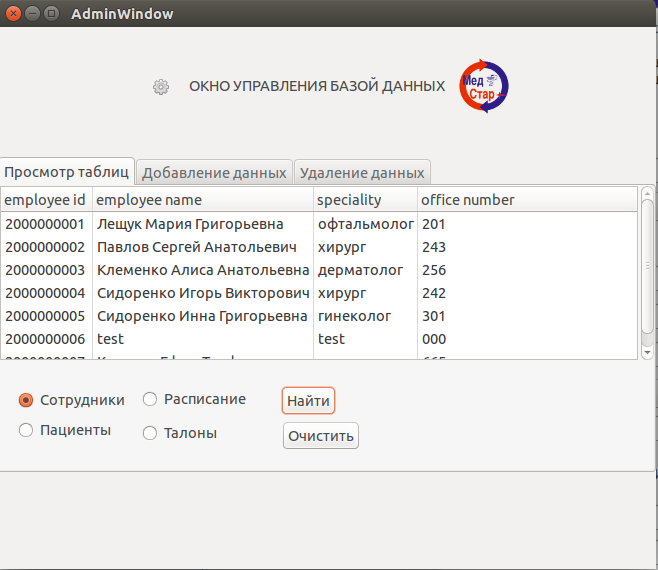
\includegraphics[width=0.9\linewidth]{admin_find}}
\caption{Просмотр данных в таблицах}
\label{admin_find:admin_find}
\end{figure}

\begin{figure}[h!]
\center{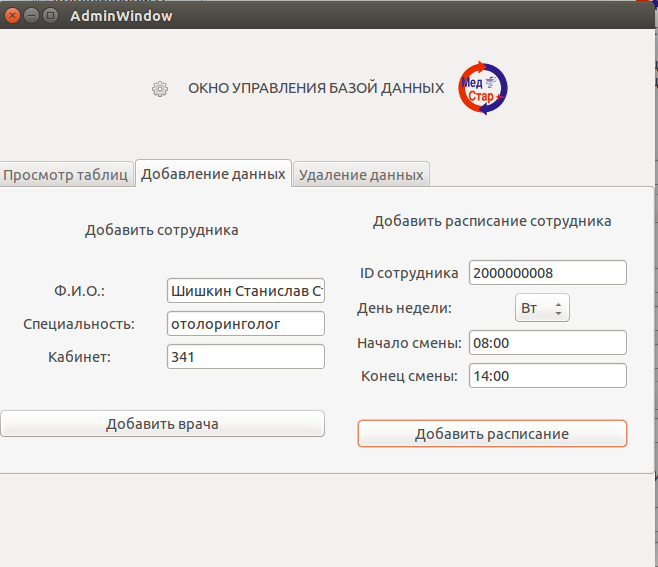
\includegraphics[width=0.9\linewidth]{admin_insert}}
\caption{Добавление данных}
\label{admin_insert:admin_insert}
\end{figure}

\begin{figure}[h!]
\center{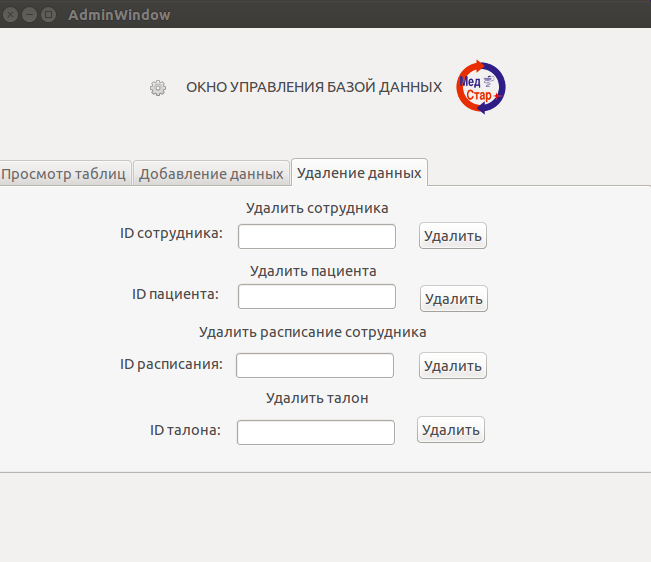
\includegraphics[width=0.7\linewidth]{admin_delete}}
\caption{Удаление данных}
\label{admin_delete:admin_delete}
\end{figure}

Необходимо правильно заполнять все поля для ввода. Если где-либо ввод осуществлен неверно, появится сообщение об ошибке ввода (рис.~\ref{err_win:err_win}), если же все действия проделаны верно --- сообщение об успешном завершении операции (рис.~\ref{suc_win:suc_win}).

\begin{figure}[h!]
\center{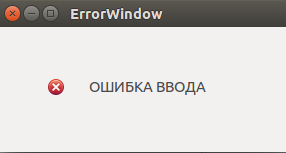
\includegraphics[width=0.5\linewidth]{err_win}}
\caption{Сообщение об ошибке ввода}
\label{err_win:err_win}
\end{figure}

\begin{figure}[h!]
\center{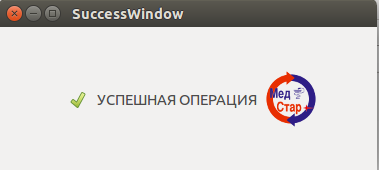
\includegraphics[width=0.5\linewidth]{suc_win}}
\caption{Сообщение об успешном завершении операции}
\label{suc_win:suc_win}
\end{figure}
